\graphicspath{{content/2_design/figures/}}
\section{Current sensor}\label{sec:current_sensor_design}
\subsubsection{Configuration}\label{sec:current_sensor_config}

The differential amplifier configuration will be used for this project for the following reasons:
\begin{itemize}
  \item The configuration is specifically designed to reject common-mode noise, which the non-inverting amp suffers from.
  \item Only 1 op-amp is needed.
  \item The design is relatively simple compared to the instrumentation amplifier.
\end{itemize}

However, a modified version with two extra capacitors will be used. Two capacitors will be added in parallel with $R_f$ and $R_g$ called $C_f$ and $C_g$ respectively. It is important that these capacitors have the same
value in order to preserve CMRR \cite{opAmpConfigurations}. It is likely, however, that one of these will be dominant due to differing resistor values, and therefore this design will only consider the filter to be first-order.
This is acceptable, however, due to the amplifier's noise-rejecting capabilities.

\subsubsection{Gain and Cutoff}
Before calculating component values, both the cutoff frequency of the RC filter, and the DC gain of the amplifier, need to be determined. The gain of the amplifier should be determined
such that, when the maximum current flows through the sense resistor, the maximum voltage is output.

First, the maximum current of the motor should be measured. This can be done by connecting the motor to a power supply (through an ammeter), stalling the motor, and reading the output current.
With a supply voltage of 6.4 V connected, the motor for this project read 740 mA, however different motors may read between 1 and 1.5 A. The average running current, however, is between 200 mA
and 300 mA. A value of $I_{max} = 1 A$ will therefore be chosen to allow for more headroom and a slightly lower gain.
Since a sense resistor of $\SI{10}{\milli\ohm}$ is to be used, the maximum voltage through this resistor will therefore be 8 mV. A gain of $\frac{3 V}{10 mV} = 300$ is therefore chosen.
Although this voltage level is small, it is expected, given that the resistance value is so small. It is also desirable, as it shows that the circuit is not "stealing" too much power from the motor itself.

The cutoff frequency $f_H$ should be selected such that the slew rate requirements are not affected, while still adequately filtering a 1 kHz noise signal. In order for the noise requirement
to be satisfied, the input signal must be attenuated by $20 \log{\frac{300 * 10 mV}{250 mV}} \approx 22 dB$. This means the cutoff should be around 100 Hz (a decade below 1 kHz).
Since the specification requires a change from 0.1 to $3 \times 0.9 = 2.7 V$ in less than 100 ms, the output should be capable of oscillating at $\frac{1}{50 ms} = 20 Hz$, which is below the designed cutoff.

Since input current of the circuit needs to be limited below 150 uA, high resistor values should be chosen:
\begin{itemize}
  \item Assuming $i_n = 0$, choose $\frac{V_{out(max)}}{R_1 + R_f} << 150 uA \therefore R_1 + R_f >> \SI{20}{\kilo\ohm}$. Choose $R_f = \SI{100}{\kilo\ohm}$.
  \item $G = \frac{R_f}{R_1} = 300 \therefore R_1 = \SI{330}{\ohm}$
  \item Choose $R_2 = R_1 = \SI{330}{\ohm}$ and $R_g = R_f = \SI{100}{\kilo\ohm}$ for differential symmetry.
  \item Since $R_{eq}$ of $C_f$ is $R_f$ and of $C_g$ is $R_g || R_2$, it is clear that $C_f$ is dominant, $\therefore C_f = \frac{1}{2 \pi \cdot R_f \cdot 100 Hz} \approx 15 nF$. Also set $C_g = 15nF$ for symmetry.
        It should be noted, however, that this technique (using time constants) is not always valid - especially in complex circuits such as these - and so these results should be checked using simulations.
\end{itemize}

\subsubsection{Circuit diagram}\label{sec:current_sensor_circuit}
The following figure details the final circuit design for the sensor and amplifier system.

\begin{figure}[h!]
  \centering
  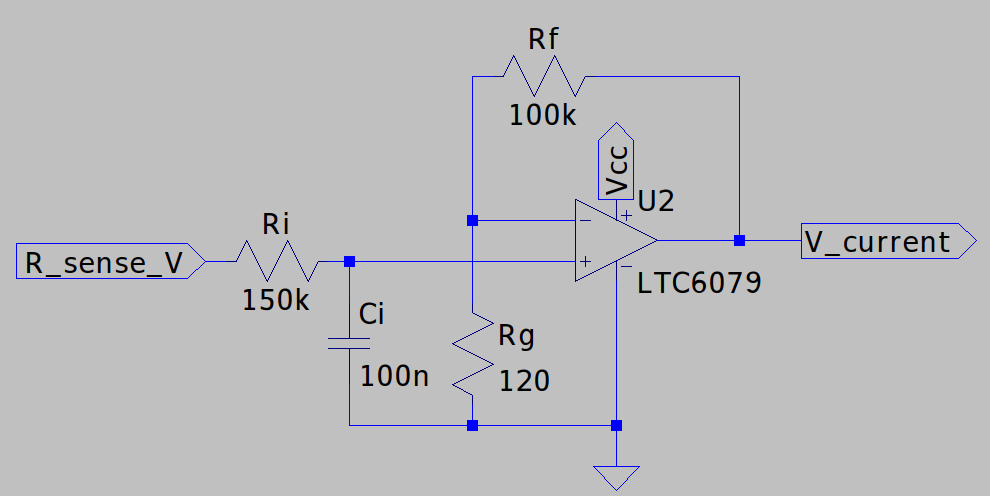
\includegraphics[width=.8\linewidth]{currentSensor_sim_circuit}
  \captionof{figure}{Circuit diagram of final configuration}  
  \label{fig:circuit-diagram}
\end{figure}

A single 5 V supply will be used. Although there are benefits to a dual rail supply, that would prove impractical in the context of the larger system.

\pagebreak
